There are two types of regulators: \textit{switching} and \textit{linear}. In
linear regulators, voltage is regulated via feedback controls. Can only handle
voltage-dropping applicatins. They are not very efficient but are noise free.
\newline
Switching regulators use transistors transfer energy via over inductors or
capacitors. This kind of regulator are much more efficient than the linear type
but also generate noise.

\subsection*{Linear regulators}
There are two types of linear regulator, shunt and series-pass.
\subsubsection*{Shunt regulator}
A shunt regulator uses a zener diode to regulate ouput voltage. It utilizes the
fact that a zener diode allows back current when subjectet to a voltage above
the \textit{zener voltage}, $V_z$. In the shunt regulator, $V_z=V_{out}$. This
type of regulator has a number of drawbacks, namely
\begin{itemize}
    \item $V_{out}$ cannot easily be chosen, it depends on available types of
zener diodes.
    \item $V_z$ changes with input voltage, $V_+$ and zener current, $I_z$. This
is given by the equation
\begin{equation}
    I_z=\frac{V_+ - V_z} {R}
\end{equation}
\item Since $I_z$ must be chosen to be large enough, using $R$, the voltage
source is running at full current all the time.
\item A high power zener is required to accommodate large load currents.
\end{itemize}
The diagram for the shunt regulator is displayed in Figure~\ref{fig:shunt}
\begin{figure}[H]
\centering
\ctikzset{bipoles/length=0.7cm}
\begin{circuitikz}\draw 
    (0,0) node[anchor=east] {}
        to[short, o-*] (1,0)
        to[zD*, v=$V_z$] (1,2)
        -- (3,2)
        to[C=1<\micro\farad>, *-*] (3,0) 
        -- (1,0)
    (0,4) node[anchor=east] {$V_+$}
        to[short, o-] (1,4)
        to[R=R, -*] (1,2)
    (5,2) node[anchor=west] {$V_{out}$}
        to[short, o-] (3,2)
    (5,0) node[anchor=west] {}
        to[short, o-] (3,0)
;
\end{circuitikz}
\caption{Shunt regulator circuit}
\label{fig:shunt}
\end{figure}
The capacitor is used for output filtering and $R$ is used to adjust $I_z$.
\subsubsection*{Series-pass regulator}
To remove the need for a power zener, one might use a series-pass regulator,
depicted in Figure~\ref{fig:spreg}. This uses an \textit{emitter follower
transistor} to regulate voltage. The output voltage is then
$V_{out}=V_{ref}-V_{BE}$. An emitter follower npn transistor has current gain but no
voltage gain. This setup has the problem that that $V_{BE}$ varies with output
current. This is alliviated by putting a op amp at the base of the transistor,
fed back from a voltage divider at the output. This also allows the circuit to
be adjusted.
\begin{figure}[H]
\centering
\begin{circuitikz} \draw
    (0,0) node[anchor=east] {}
        to[short, o-o] (7,0)
    % Transistor
    (2,6) node[npn, rotate=90, anchor=C] (npn) {}
    (npn.B) node[anchor=north] {}
    (npn.C) node[anchor=west] {}
    (npn.E) node[anchor=east] {}
    (0,6) node[anchor=east] {$V_+$}
        to[short, o-] (npn.C) 
    (npn.E) to[short, -o] (6,6)
        to[R=R1, *-*] (6,4)
        to[R=R2, *-*] (6,0)
    (4,4) node[op amp, xscale=-0.5, yscale=0.5, anchor=-] (opamp) {}
    (6,4) node[anchor=east] {}
        to[short, *-] (opamp.-)
    (5,0) node[anchor=south] {}
        to[V=Vref] (5,2)
        -| (opamp.+)
    (opamp.out) node[] {}
        to[short] (npn.B)
    (7,6) node[yshift=0.5cm] {$V_{out}$}
        to[short, o-] (6,6)
       
;
\end{circuitikz}
\caption{Simple series-pass regulator.}
\ref{fig:spreg}
\end{figure}

\subsection*{Switching regulators}
There are several types of switched regulators. These can both switch up or down
the voltage.

\subsubsection*{Step-Down (Buck/Forward mode) Converter}
A step down converter (Figure~\ref{fig:buck}uses an inductor and a switch to make the output voltage
lower than the input voltage. It can generate high output power, up to kW and
produces less ripple than a Boost mode converter.
\begin{figure}[H]
\centering
\begin{circuitikz}[american inductors] \draw
    (0,0) node[] {}
        to[short, o-o] (7,0)
    (0,3) node[anchor=east] {$V_{in}$}
    to[short, o-] (0,3)
        to[switch, -*] (3,3) 
        to[L=L, *-*] (6,3)
        to[C=C, *-*] (6,0)
        -- (3,0)
        to[D*=D, *-*] (3,3)
    (7,3) node[anchor=west] {$V_{out}$}
        to[short, o-] (6,3)
;
\end{circuitikz}
\caption{Step down converter.}
\ref{fig:buck}
\end{figure}

It operates in two stages. I the first stage, the
switch is closed and the inductor is charged . In the second stage, the switch
is open and the inductor is discharged via the load and through the diode. There
are some losses over the diode, so a second switch might be used there instead.
The circuit is then running in \textit{synchronus mode}. The capacitor $C$ is
used for smoothing the output voltage. The output voltage is dependent on the
PWM duty cycle, $D$, and is simply
\begin{equation}
    V_{out} = DV_{in}.
\end{equation}
Assuming ideal components, the input power must equal the output power and
therefore
\begin{equation}
    I_{in} = I_{out}\frac {V_{out}} {V_{in}}
\end{equation}
must hold. Also, the output current is equal to the difference between the
minimum and the maximum current over the switch, $\Delta I$, 
\begin{equation}
    I_{out} = \Delta I_{in}
\end{equation}
The switching is shown in Figure~\ref{fig:buckswitch}
\begin{figure}[H]
    \centering
    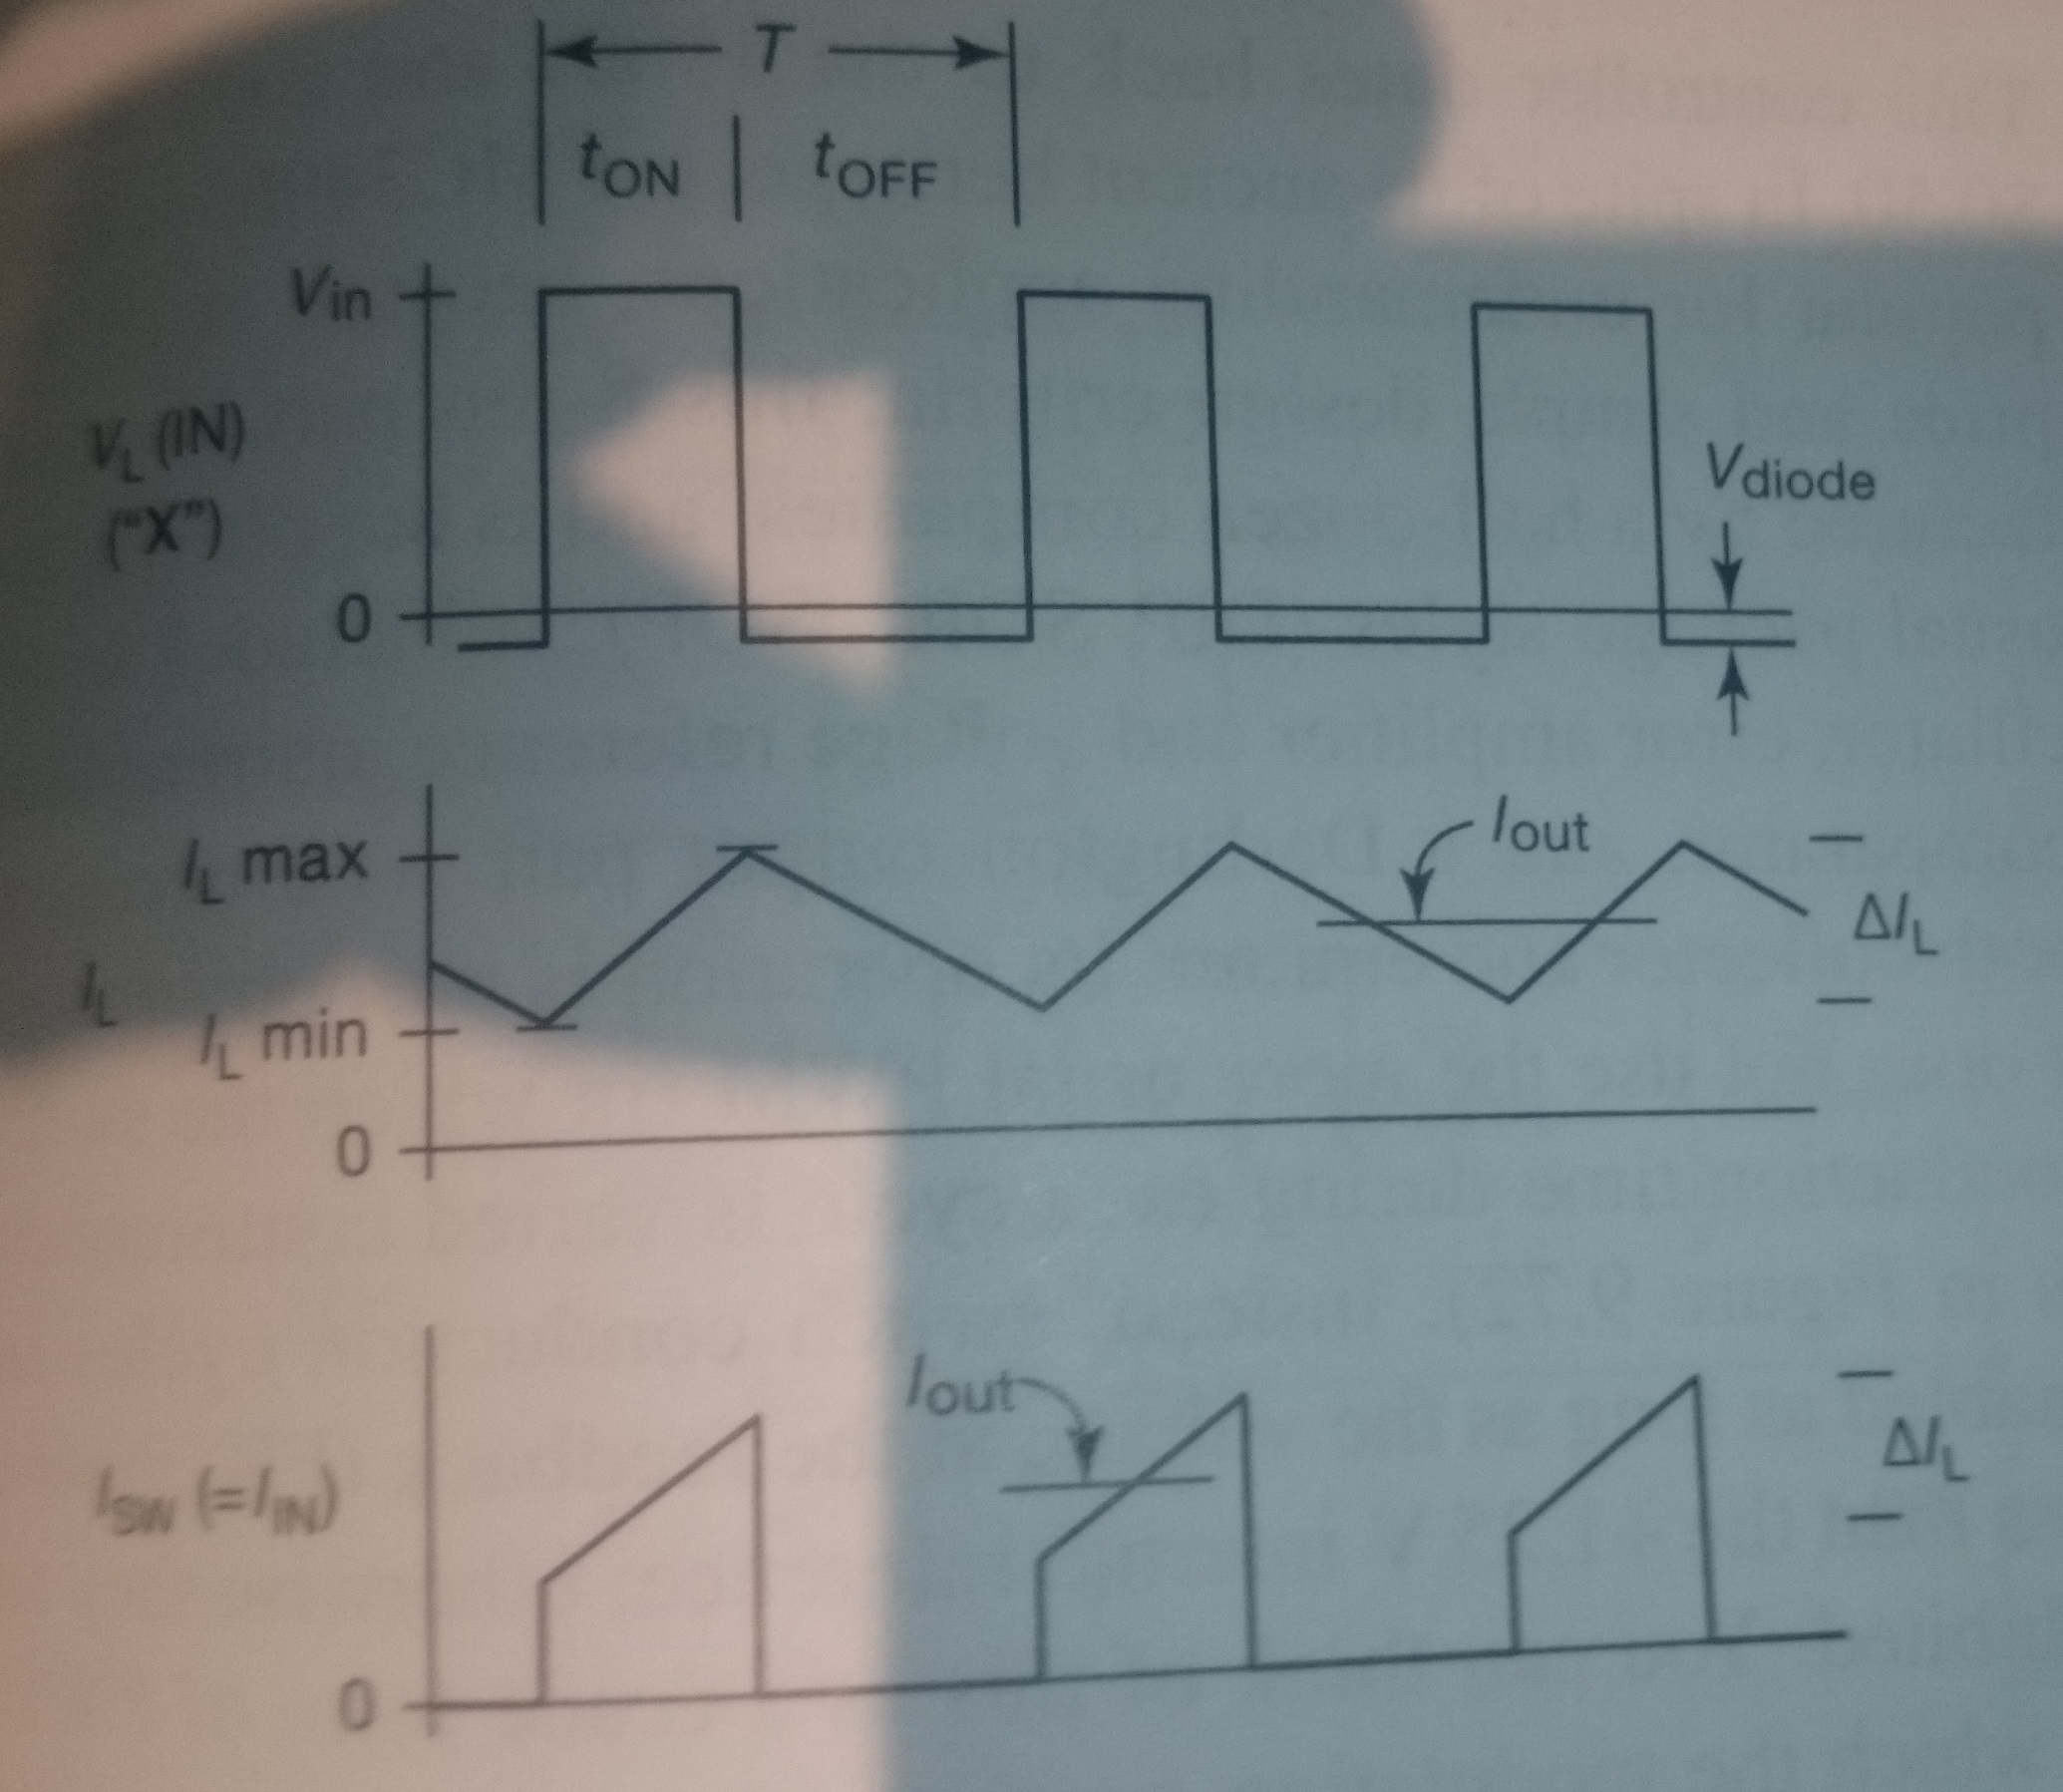
\includegraphics[height=3cm]{./figures/buckswitch.jpg}
    \caption{Swithcing of Buck regulator}
    \label{fig:buckswitch}
\end{figure}

\subsubsection*{Step up (Boost mode) converter}
A Boost mode converter is a rearranged Buck converter, shown in
Figure~\ref{fig:boost}. The boost mode converter
delivers higher output voltage than the input voltage. 
\begin{figure}[H]
\centering
\begin{circuitikz}[american inductors] \draw
    (0,0) node[] {}
        to[short, o-o] (7,0)
    (0,3) node[anchor=east] {$V_{in}$}
    to[short, o-] (0,3)
        to[L=L, -*] (3,3) 
        to[D*=D, *-*] (6,3)
        to[C=C, *-*] (6,0)
        -- (3,0)
        to[switch, *-*] (3,3)
    (7,3) node[anchor=west] {$V_{out}$}
        to[short, o-] (6,3)
;
\end{circuitikz}
\caption{Step up converter.}
\ref{fig:boost}
\end{figure}
It does so by charging the inductor when the switch is closed. When the switch
is opened, the voltage before the diode goes up and the inductor dumps it's
current into the diode. The regulator can be run in either continuous or
discontinuous mode, during which the current drops down to 0 between switching.
The current over the inductor (in current) is given by
\begin{equation}
    I_L = DV_{in} \frac{T} {L}.
\end{equation}
Running in discontinuous current mode (DCM) causes bigger ripple than continuous
mode (CCM), though CCM regulators can get unstable.

\subsubsection*{Isolated converters}
There are also galvanically isolated converters. These exhibit positive traits,
such as built in filtering and good in/output isolation. The isolation can lead
to problems with ground since in- and output cannot share the same ground. They
are also expensive.

\subsection*{Types of capacitors}
There are several types of capacitors. A short list of pros and cons of
different types are listed below in Table~\ref{tab:caps}
\begin{table}[H]
    \centering
    \begin{tabular}{| p{2cm} | p{2cm} | p{2cm} | p{4cm} |}
    \hline
    Type & Pros & Cons & Application \\
    \hline
    Metal foil & Low carbon, less fire risk & Big size & - \\
    \hline
    Polypropylene & Low loss, high stability & Big size, Costly & - \\
    \hline
    Polyester & Small, low price & Low performance & - \\
    \hline
    Polyphenylene Sulphite & High temp, low loss, high stability & Low voltage &
    - \\
    \hline
    Plastic foil & Low cost, low resistance & Low freq, stability & Decoupling,
    Filters and timing circuits. \\
    \hline
    Ceramic & High stability, temp, freq, time, voltage & Cost, Low F & High
    freq \\
    \hline
    Electrolyte & High C anv V, Dry: Age & Polar, Dry: Low V & Wet: Power
    supplies \\
    \hline
    Tantalum & - & Small F & - \\
    \hline
\end{tabular}
\caption{Different types of capacitors}
\label{tab:cap}
\end{table}
The quality of a capacitor has low damping. Given damping factor $d$, quality is
given by
\begin{equation}
    Q = \frac {1} {d}
\end{equation}
where 
\begin{equation}
    d = \frac {R_s} {X_c}.
\end{equation}
The impedance of a capacitor is given by
\begin{equation}
    X_c = \frac {1} {\omega C}
\end{equation}
